\chapter{Generazione Stocastica di Nuovi Scenari (Validazione del VAE)}
\label{ch:generazione_stocastica}

\section{Campionamento dallo spazio latente: dal prior al block-bootstrap storico}
\label{sec:block_bootstrap}

Come discusso nel Capitolo~\ref{ch:modelli_generativi} (\S\ref{sec:vae}), la regolarizzazione imposta dalla Divergenza di Kullback-Leibler rende in linea di principio possibile generare nuove matrici di correlazione campionando direttamente un vettore casuale $\mathbf{z}_{\text{sim}} \sim \mathcal{N}(\mathbf{0}, \mathbf{I})$ dal \emph{prior} e decodificandolo. Tuttavia, l'obiettivo di questo lavoro non è produrre uno scenario plausibile qualsiasi, bensì \textbf{prevedere la struttura di correlazione a un orizzonte di un mese} a partire dallo stato di mercato osservato oggi (Capitolo~\ref{ch:matrici_finanziarie}, \S\ref{sec:markowitz}). Per questo motivo, la procedura di generazione effettivamente adottata sostituisce il semplice campionamento dal \emph{prior} con una tecnica di \textbf{block-bootstrap storico nello spazio latente}, che ancora la generazione stocastica alla dinamica recente del mercato pur sfruttando la medesima regolarità topologica dello spazio latente descritta nel Capitolo~\ref{ch:modelli_generativi}.

La procedura, applicata al modello VAE a 20 dimensioni latenti nel dominio Cholesky con loss di Jeffreys (\texttt{VAE\_20dim\_cholesky\_06\_loss}, lo stesso modello impiegato per il confronto del Capitolo~\ref{ch:analisi_compressione}), si articola nei seguenti passaggi:
\begin{enumerate}
    \item \textbf{Ricostruzione della traiettoria latente storica.} L'encoder del VAE già addestrato viene applicato all'intera serie storica delle matrici di correlazione calcolate con passo giornaliero ($\text{stride}=1$, a differenza dello stride di 10 giorni usato per l'addestramento, si veda il Capitolo~\ref{ch:preprocessing}), producendo una traiettoria latente continua $\{\mathbf{z}_t\}_{t=1}^{T}$ con $T=4124$ osservazioni giornaliere.
    \item \textbf{Calcolo degli incrementi giornalieri.} Si calcola la sequenza degli incrementi $\Delta\mathbf{z}_t = \mathbf{z}_t - \mathbf{z}_{t-1}$, che rappresenta la variazione giorno-su-giorno osservata nello spazio latente durante l'intero periodo storico.
    \item \textbf{Campionamento a blocchi.} Per generare ciascuno scenario sintetico, si estrae casualmente un blocco di 21 incrementi giornalieri consecutivi (corrispondenti a un mese lavorativo) dalla sequenza storica $\{\Delta\mathbf{z}_t\}$ e se ne calcola la somma cumulata $\delta\mathbf{z}$.
    \item \textbf{Proiezione a un mese.} Il salto latente campionato viene sommato allo stato attuale $\mathbf{z}_{\text{oggi}}$ (l'ultima osservazione della traiettoria storica), ottenendo lo stato latente previsto $\mathbf{z}_{\text{futuro}} = \mathbf{z}_{\text{oggi}} + \delta\mathbf{z}$.
    \item \textbf{Decodifica e ricostruzione PSD.} Il Decoder produce il fattore di Cholesky corrispondente a $\mathbf{z}_{\text{futuro}}$, da cui si ricostruisce la matrice di correlazione sintetica tramite $\mathbf{C} = \mathbf{L}\mathbf{L}^T$ e normalizzazione, garantendone la semidefinita positività per costruzione (Capitolo~\ref{ch:modelli_generativi}, \S\ref{sec:vae}).
\end{enumerate}

Ripetendo il campionamento a blocchi un numero $N$ di volte (in questo lavoro, $N=100$ e $N=1000$), si ottiene un insieme di scenari sintetici a un mese di distanza, ciascuno ancorato allo stesso stato di partenza $\mathbf{z}_{\text{oggi}}$ ma diversificato dalla variabilità storica campionata a blocchi.

\begin{figure}[h!]
\centering
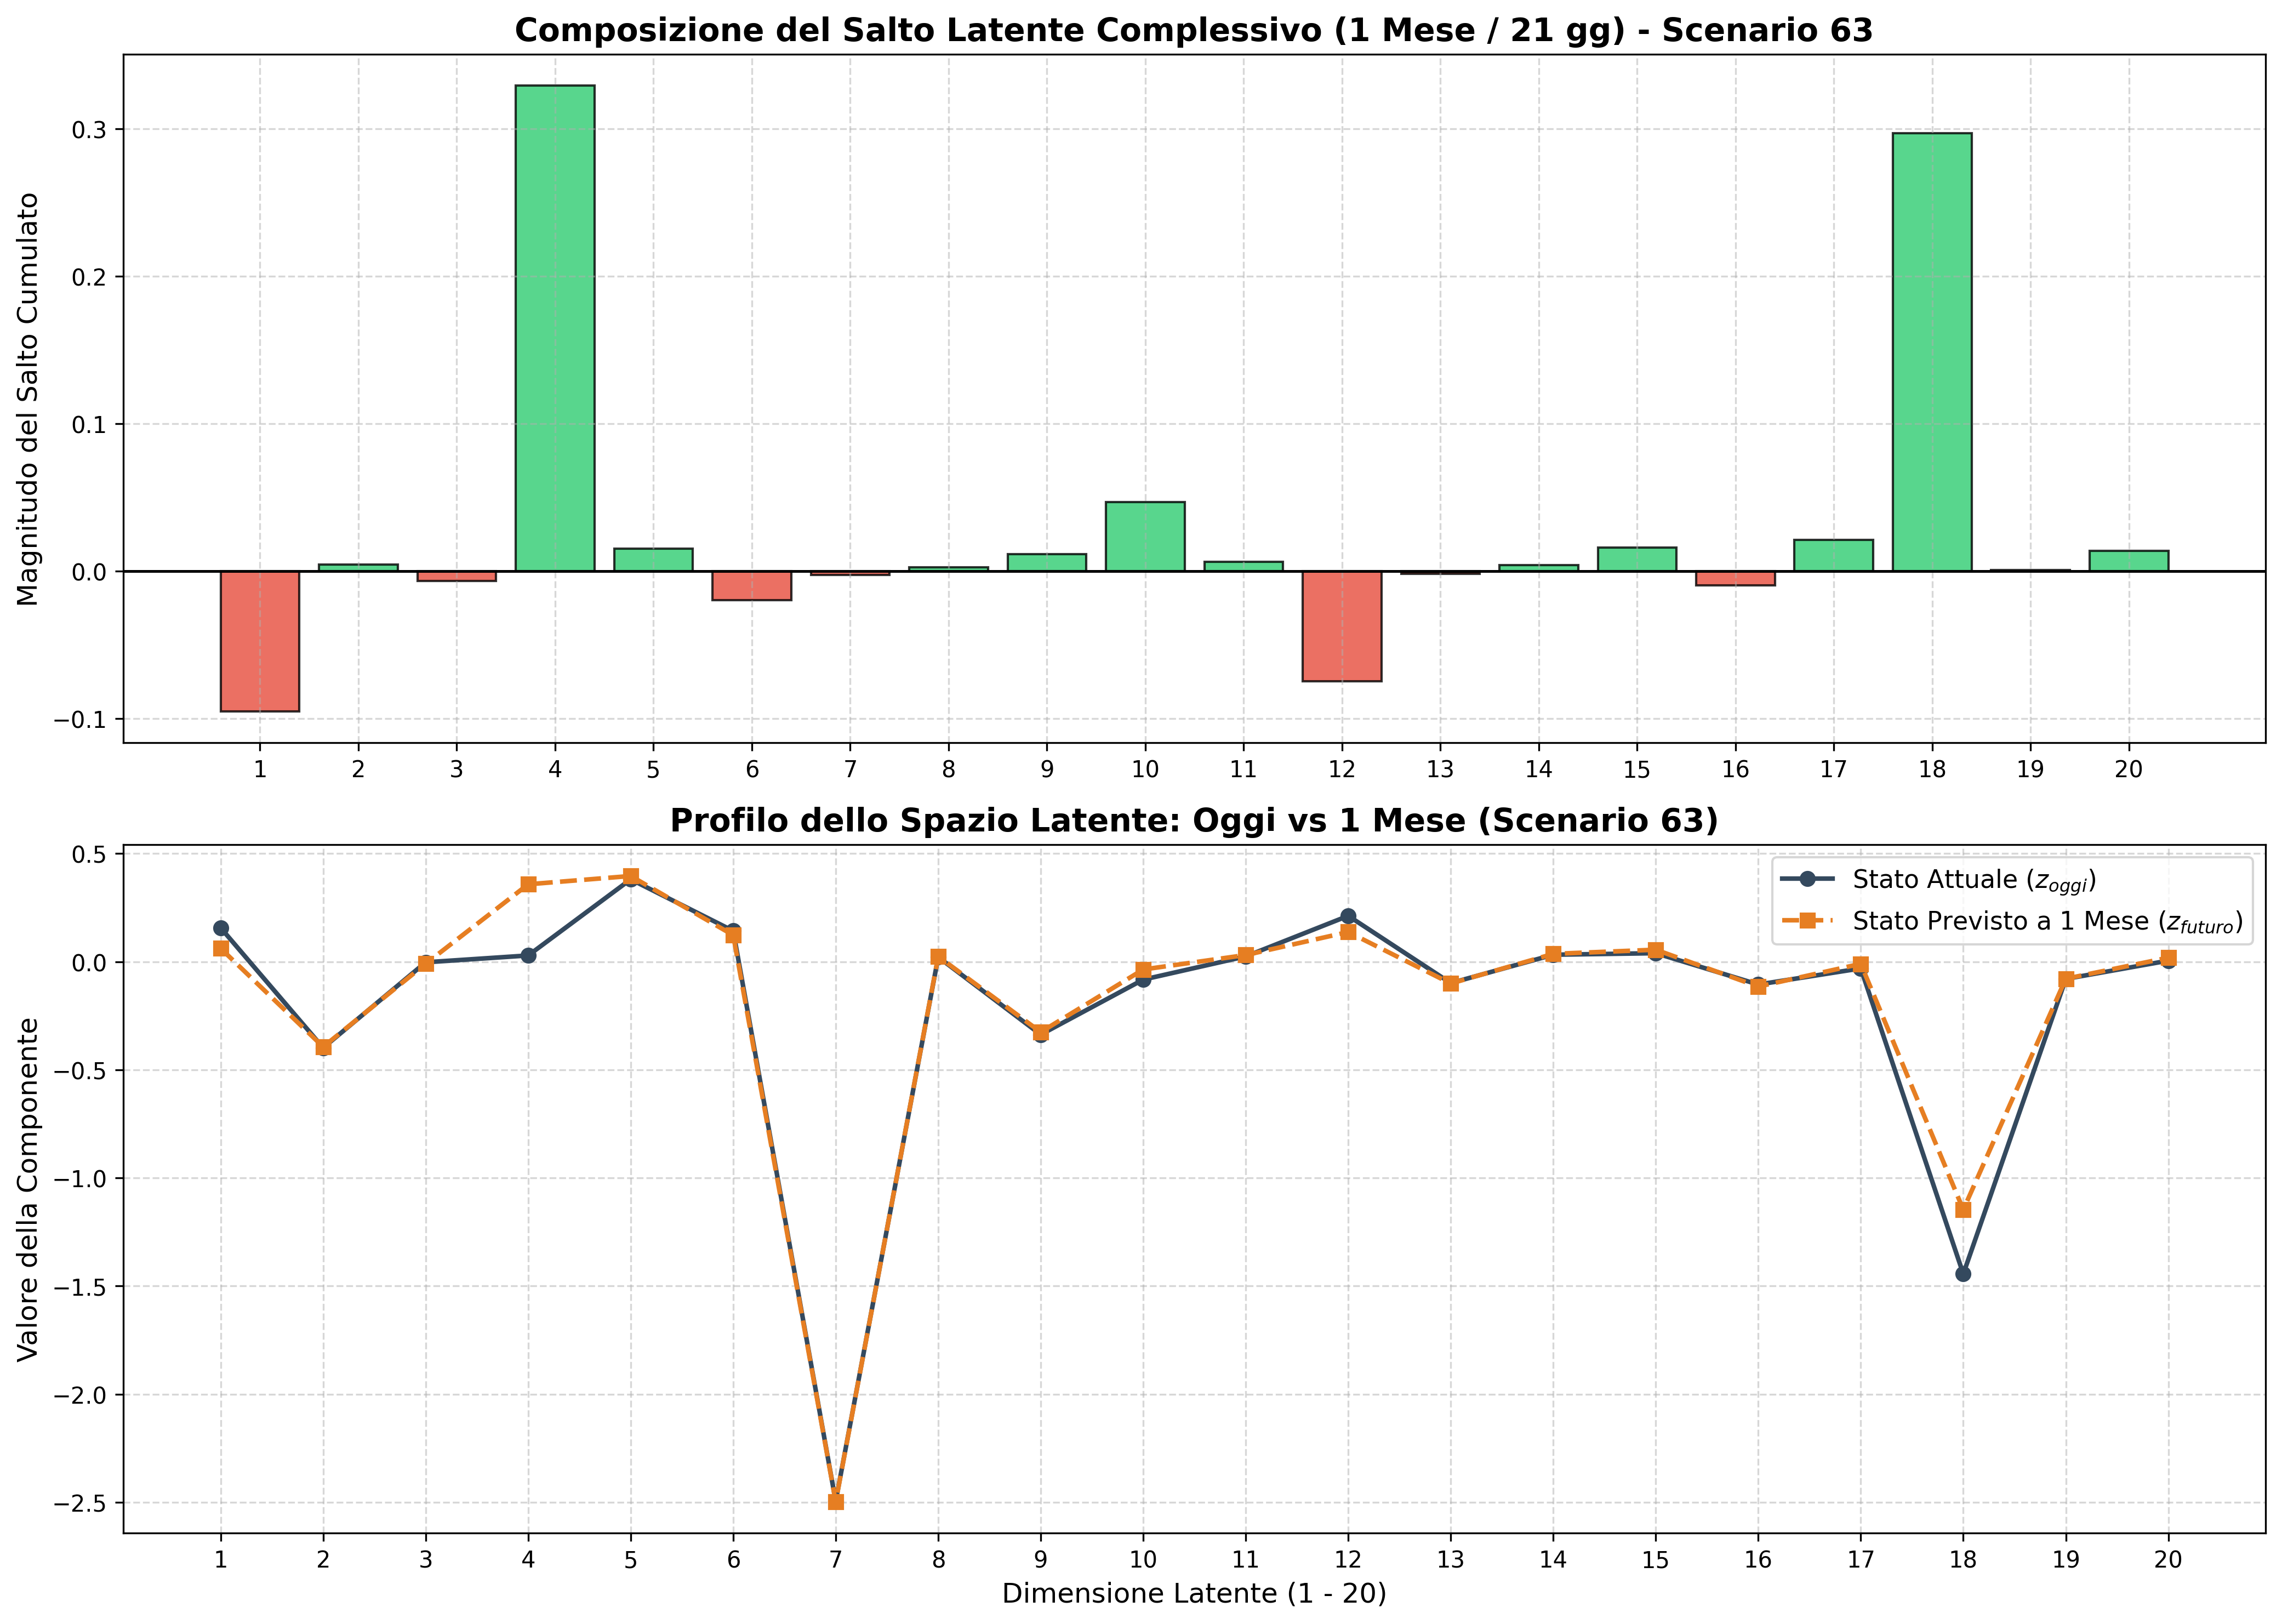
\includegraphics[width=0.85\textwidth]{./Pictures/capitolo8/fig_block_bootstrap_latente.png}
\caption{Illustrazione della procedura di block-bootstrap per uno scenario sintetico (\emph{Scenario 63} tra i 1000 generati): in alto, la composizione del salto latente cumulato sulle 20 dimensioni; in basso, il confronto tra lo stato attuale $\mathbf{z}_{\text{oggi}}$ e lo stato previsto a un mese $\mathbf{z}_{\text{futuro}}$.}
\label{fig:block_bootstrap}
\end{figure}

La Figura~\ref{fig:block_bootstrap} illustra la composizione del salto latente per uno degli scenari generati: si osserva come solo alcune dimensioni latenti (tipicamente 2--4 su 20) contribuiscano in modo sostanziale allo spostamento complessivo, mentre le restanti rimangono pressoché invariate rispetto allo stato attuale --- un comportamento coerente con la struttura dello spazio latente appreso dal VAE, in cui poche direzioni concentrano la maggior parte della variabilità informativa del mercato.

\section{Verifica dei cinque fatti stilizzati sulle matrici generate}
\label{sec:verifica_stylized_facts_generate}

Per validare la plausibilità economico-finanziaria delle matrici sintetiche prodotte, ciascuno scenario generato viene confrontato con la matrice di correlazione osservata oggi sulla base dei cinque fatti stilizzati introdotti nel Capitolo~\ref{ch:stylized_facts}. Lo scenario qui presentato in dettaglio (\emph{Scenario 63}, tra i 1000 generati dal modello \texttt{VAE\_20dim\_cholesky\_06\_loss}) è stato scelto perché si colloca al 95\textdegree\ percentile lungo il primo asse principale della nuvola di scenari generati (che spiega il 23.4\% della varianza totale, Figura~\ref{fig:analisi_statistica}): non è quindi uno scenario arbitrario o "comodo", ma uno scenario di coda, rappresentativo di una plausibile evoluzione di mercato relativamente pronunciata rispetto allo stato attuale.

\begin{figure}[h!]
\centering
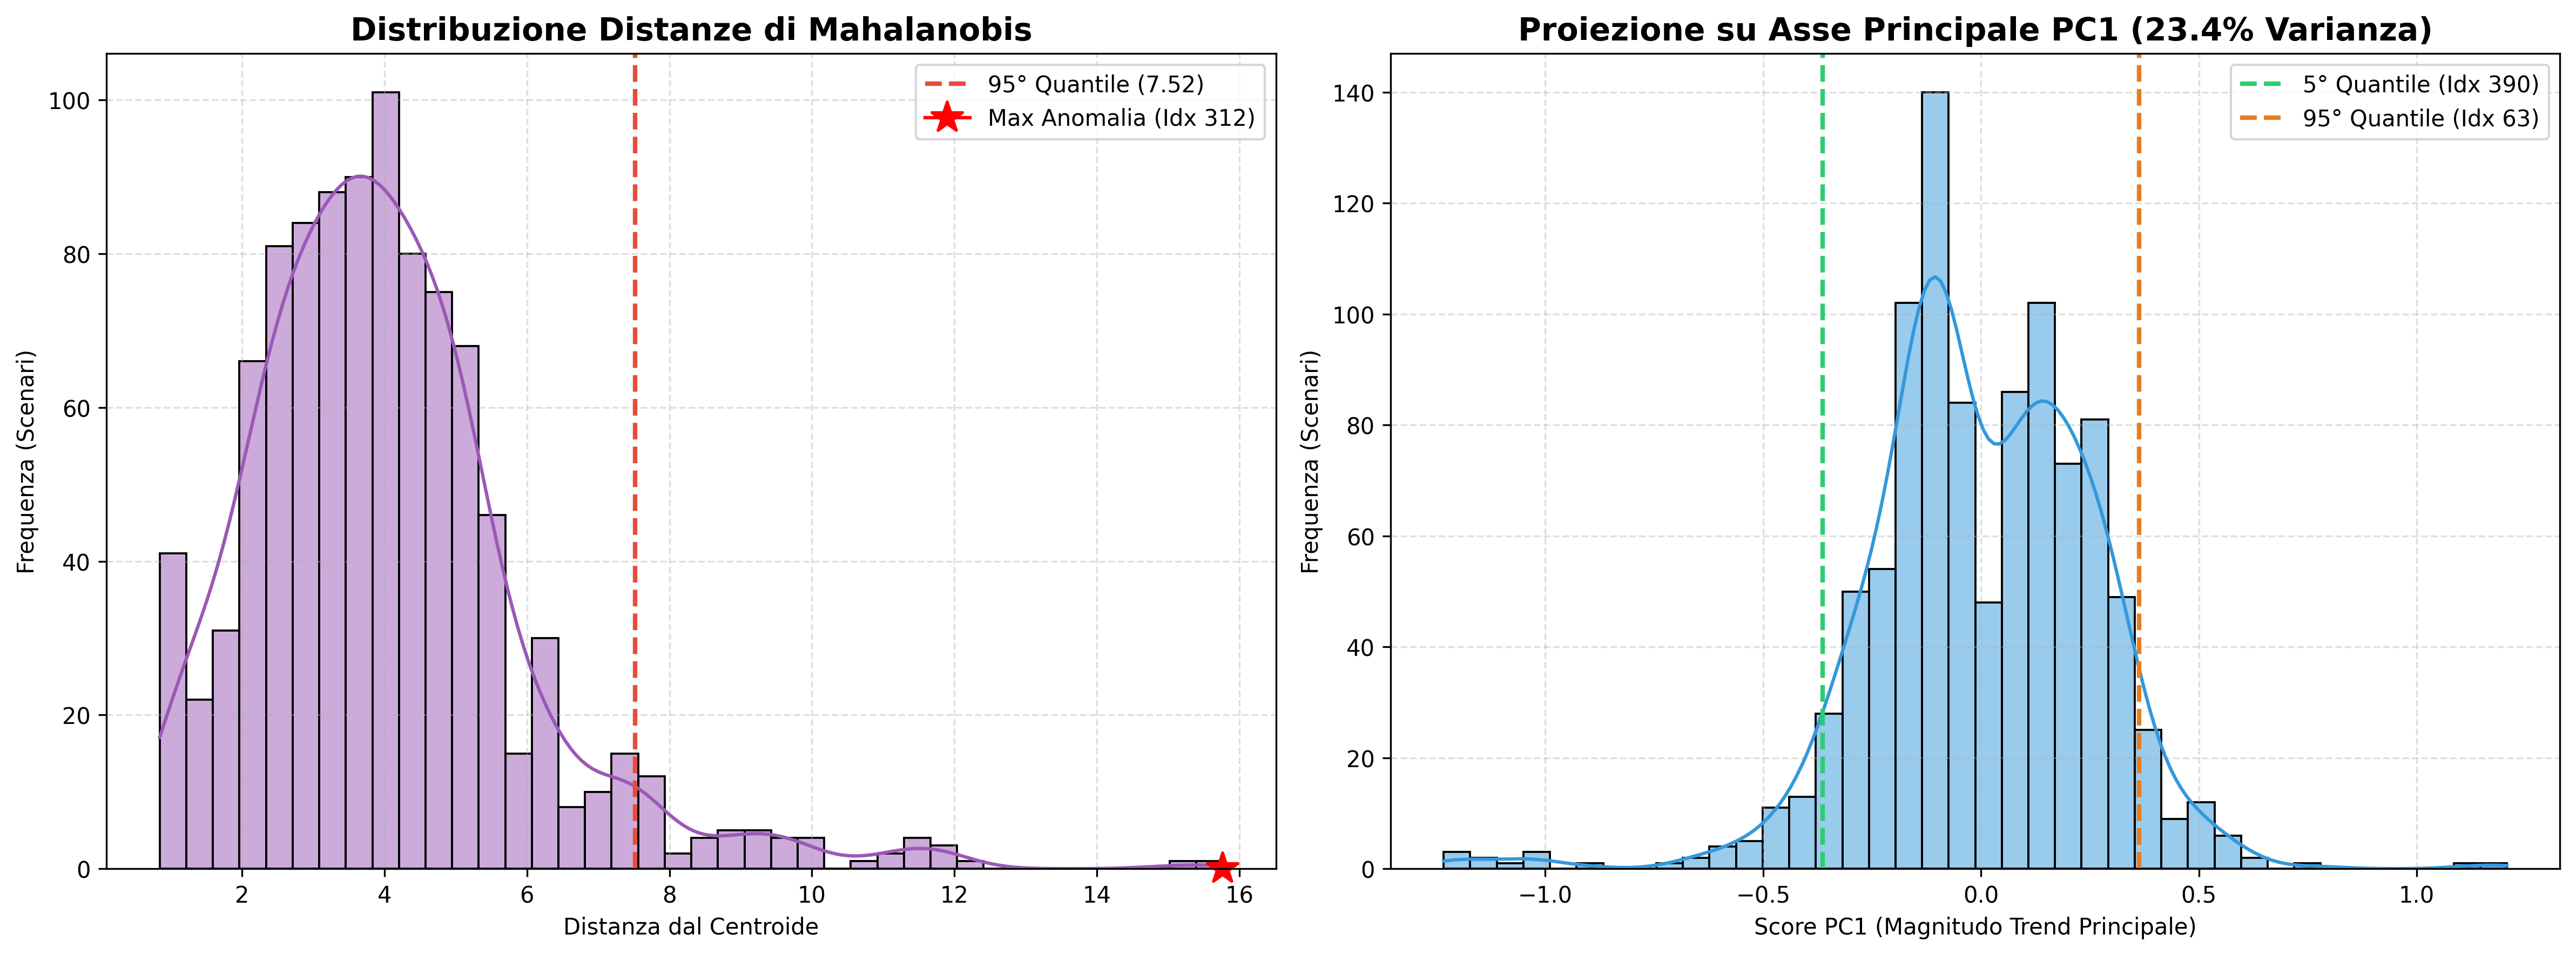
\includegraphics[width=0.95\textwidth]{./Pictures/capitolo8/fig_analisi_statistica_1000_scenari.png}
\caption{Analisi statistica della nuvola di 1000 scenari generati: distribuzione delle distanze di Mahalanobis dal centroide (sinistra) e proiezione sul primo asse principale (destra). Lo Scenario 63, oggetto dell'analisi di dettaglio, si colloca al 95\textdegree\ percentile lungo il primo asse.}
\label{fig:analisi_statistica}
\end{figure}

\paragraph{Distribuzione pairwise.} La distribuzione dei coefficienti di correlazione dello scenario sintetico (Figura~\ref{fig:pairwise_generato}) mantiene lo spostamento verso valori positivi osservato nel mercato reale: media $0.4635$ e mediana $0.4711$ per lo scenario generato, contro $0.4512$ e $0.4593$ della matrice odierna --- coerenti, per ordine di grandezza, con quanto verificato sulla matrice di esempio analizzata nel Capitolo~\ref{ch:stylized_facts}.

\begin{figure}[h!]
\centering
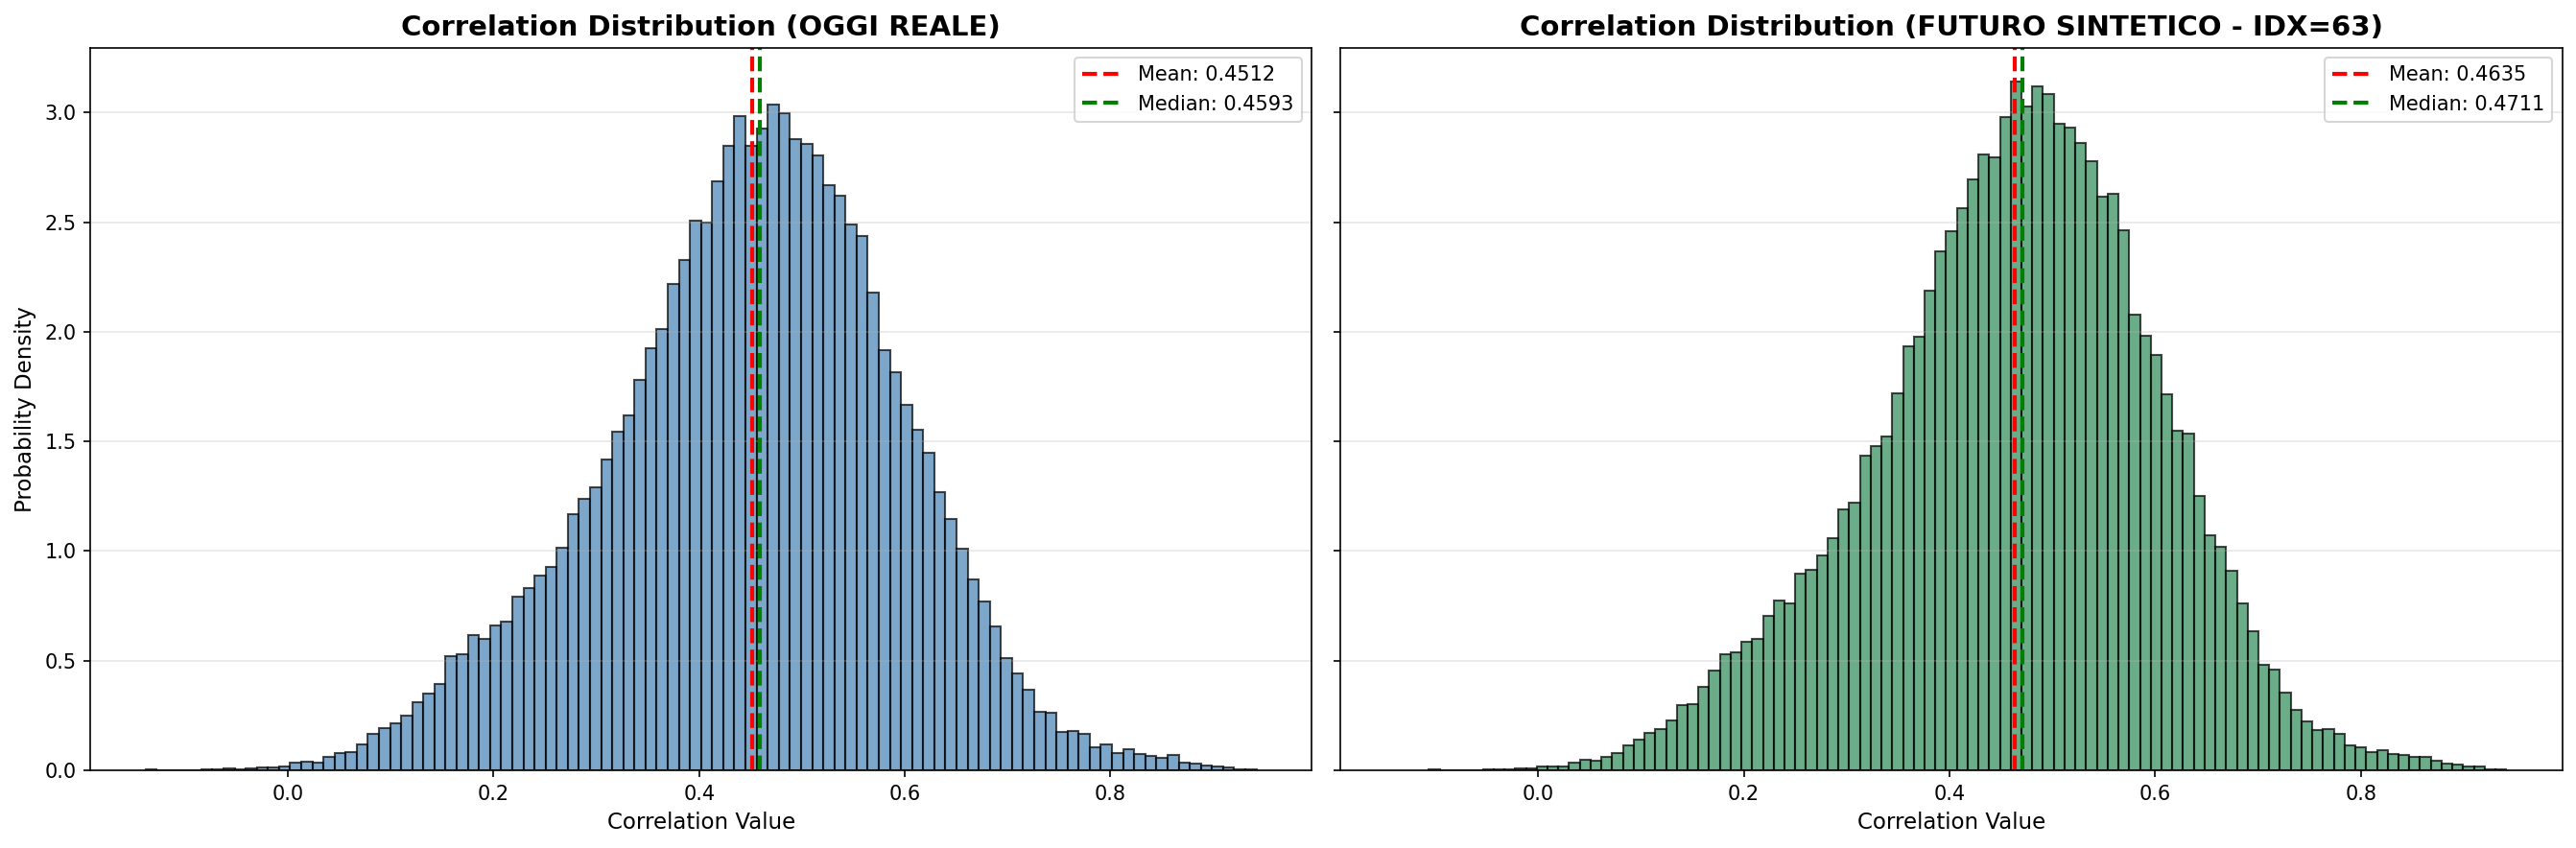
\includegraphics[width=0.95\textwidth]{./Pictures/capitolo8/fig_pairwise_distribution_generato.png}
\caption{Confronto tra la distribuzione dei coefficienti \emph{pairwise} della matrice odierna (sinistra) e della matrice sintetica a un mese (destra).}
\label{fig:pairwise_generato}
\end{figure}

\paragraph{Spettro e distribuzione di Marchenko-Pastur.} Lo spettro della matrice generata (Figura~\ref{fig:mp_generato}) preserva la struttura a tre componenti descritta nel Capitolo~\ref{ch:stylized_facts}: l'autovalore di mercato rimane dominante e di ordine di grandezza confrontabile ($169.1$ per la matrice odierna, $173.2$ per lo scenario generato), e lo stesso numero di autovalori settoriali (nove) supera il limite superiore teorico di Marchenko-Pastur in entrambe le matrici.

\begin{figure}[h!]
\centering
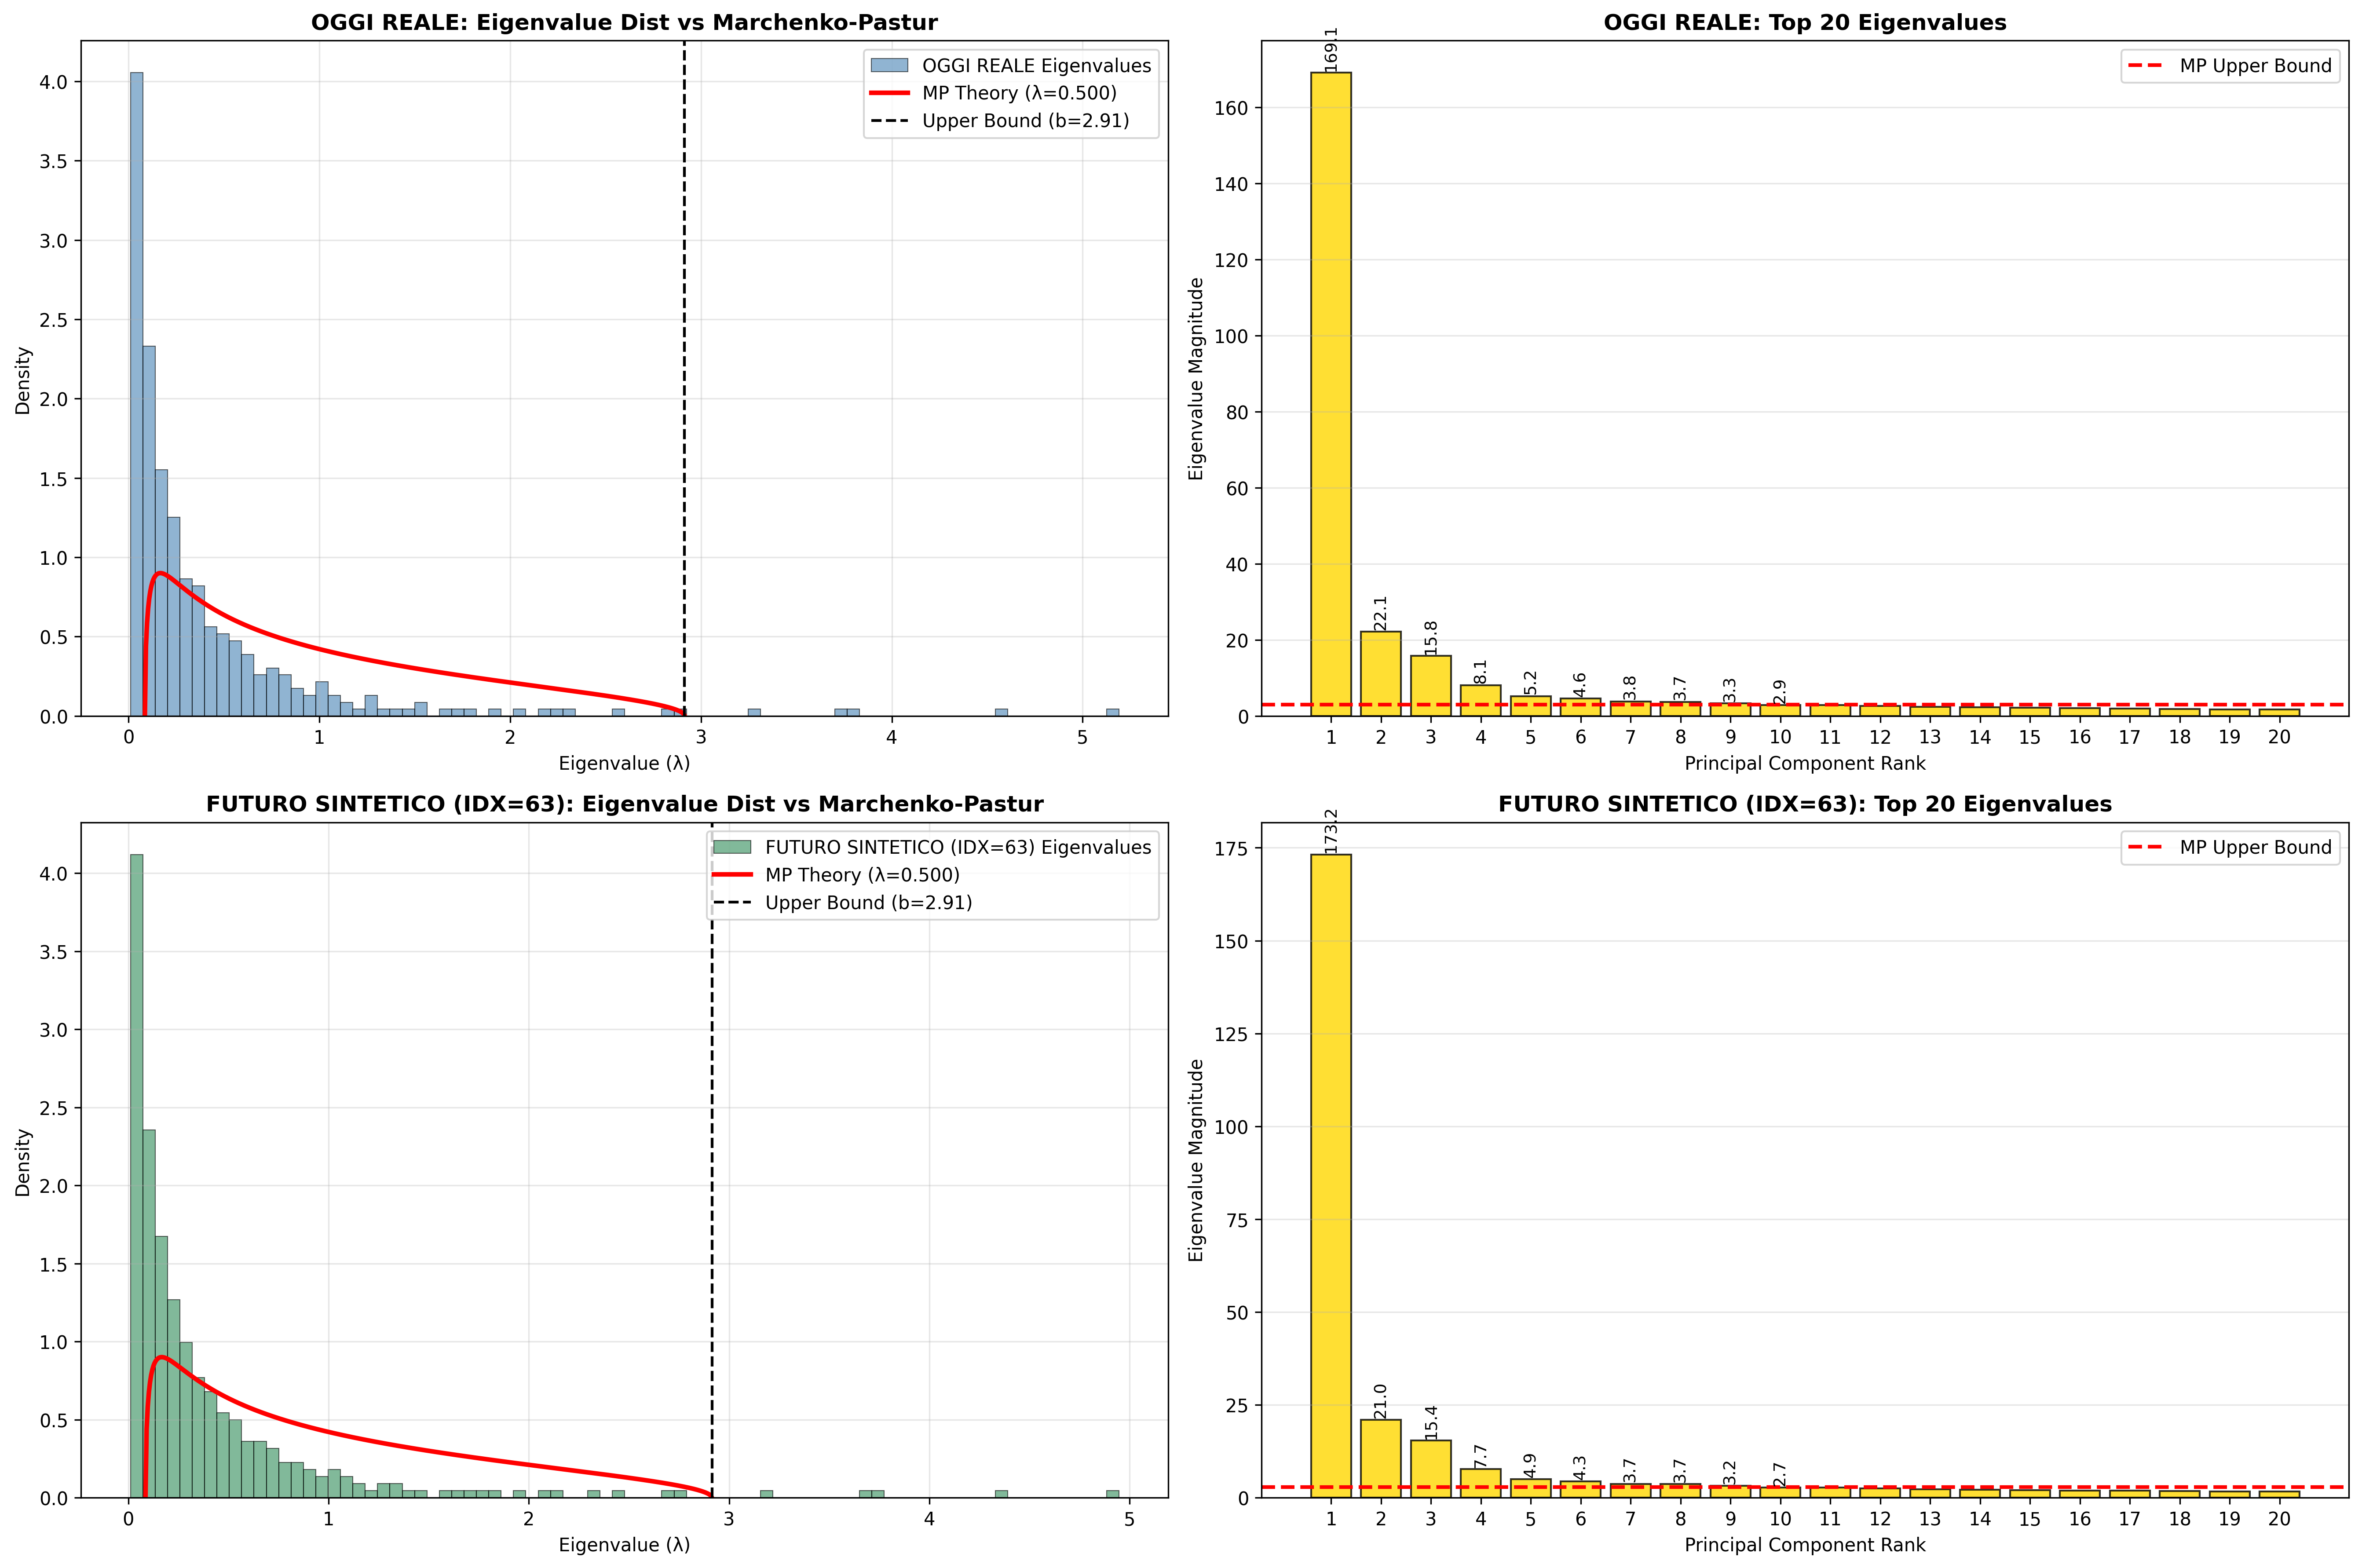
\includegraphics[width=0.95\textwidth]{./Pictures/capitolo8/fig_marchenko_pastur_generato.png}
\caption{Spettro degli autovalori della matrice odierna (in alto) e della matrice sintetica (in basso) confrontato con la distribuzione teorica di Marchenko-Pastur.}
\label{fig:mp_generato}
\end{figure}

\paragraph{Proprietà di Perron-Frobenius.} Il primo autovettore (\emph{market mode}) della matrice sintetica presenta componenti tutte dello stesso segno, in accordo con la proprietà di Perron-Frobenius, con una similarità coseno rispetto all'autovettore della matrice odierna pari a $0.9999$ (Figura~\ref{fig:pf_generato}); anche il secondo e il terzo autovettore (\emph{sector mode}) risultano preservati con similarità coseno rispettivamente di $0.9893$ e $0.9883$.

\begin{figure}[h!]
\centering
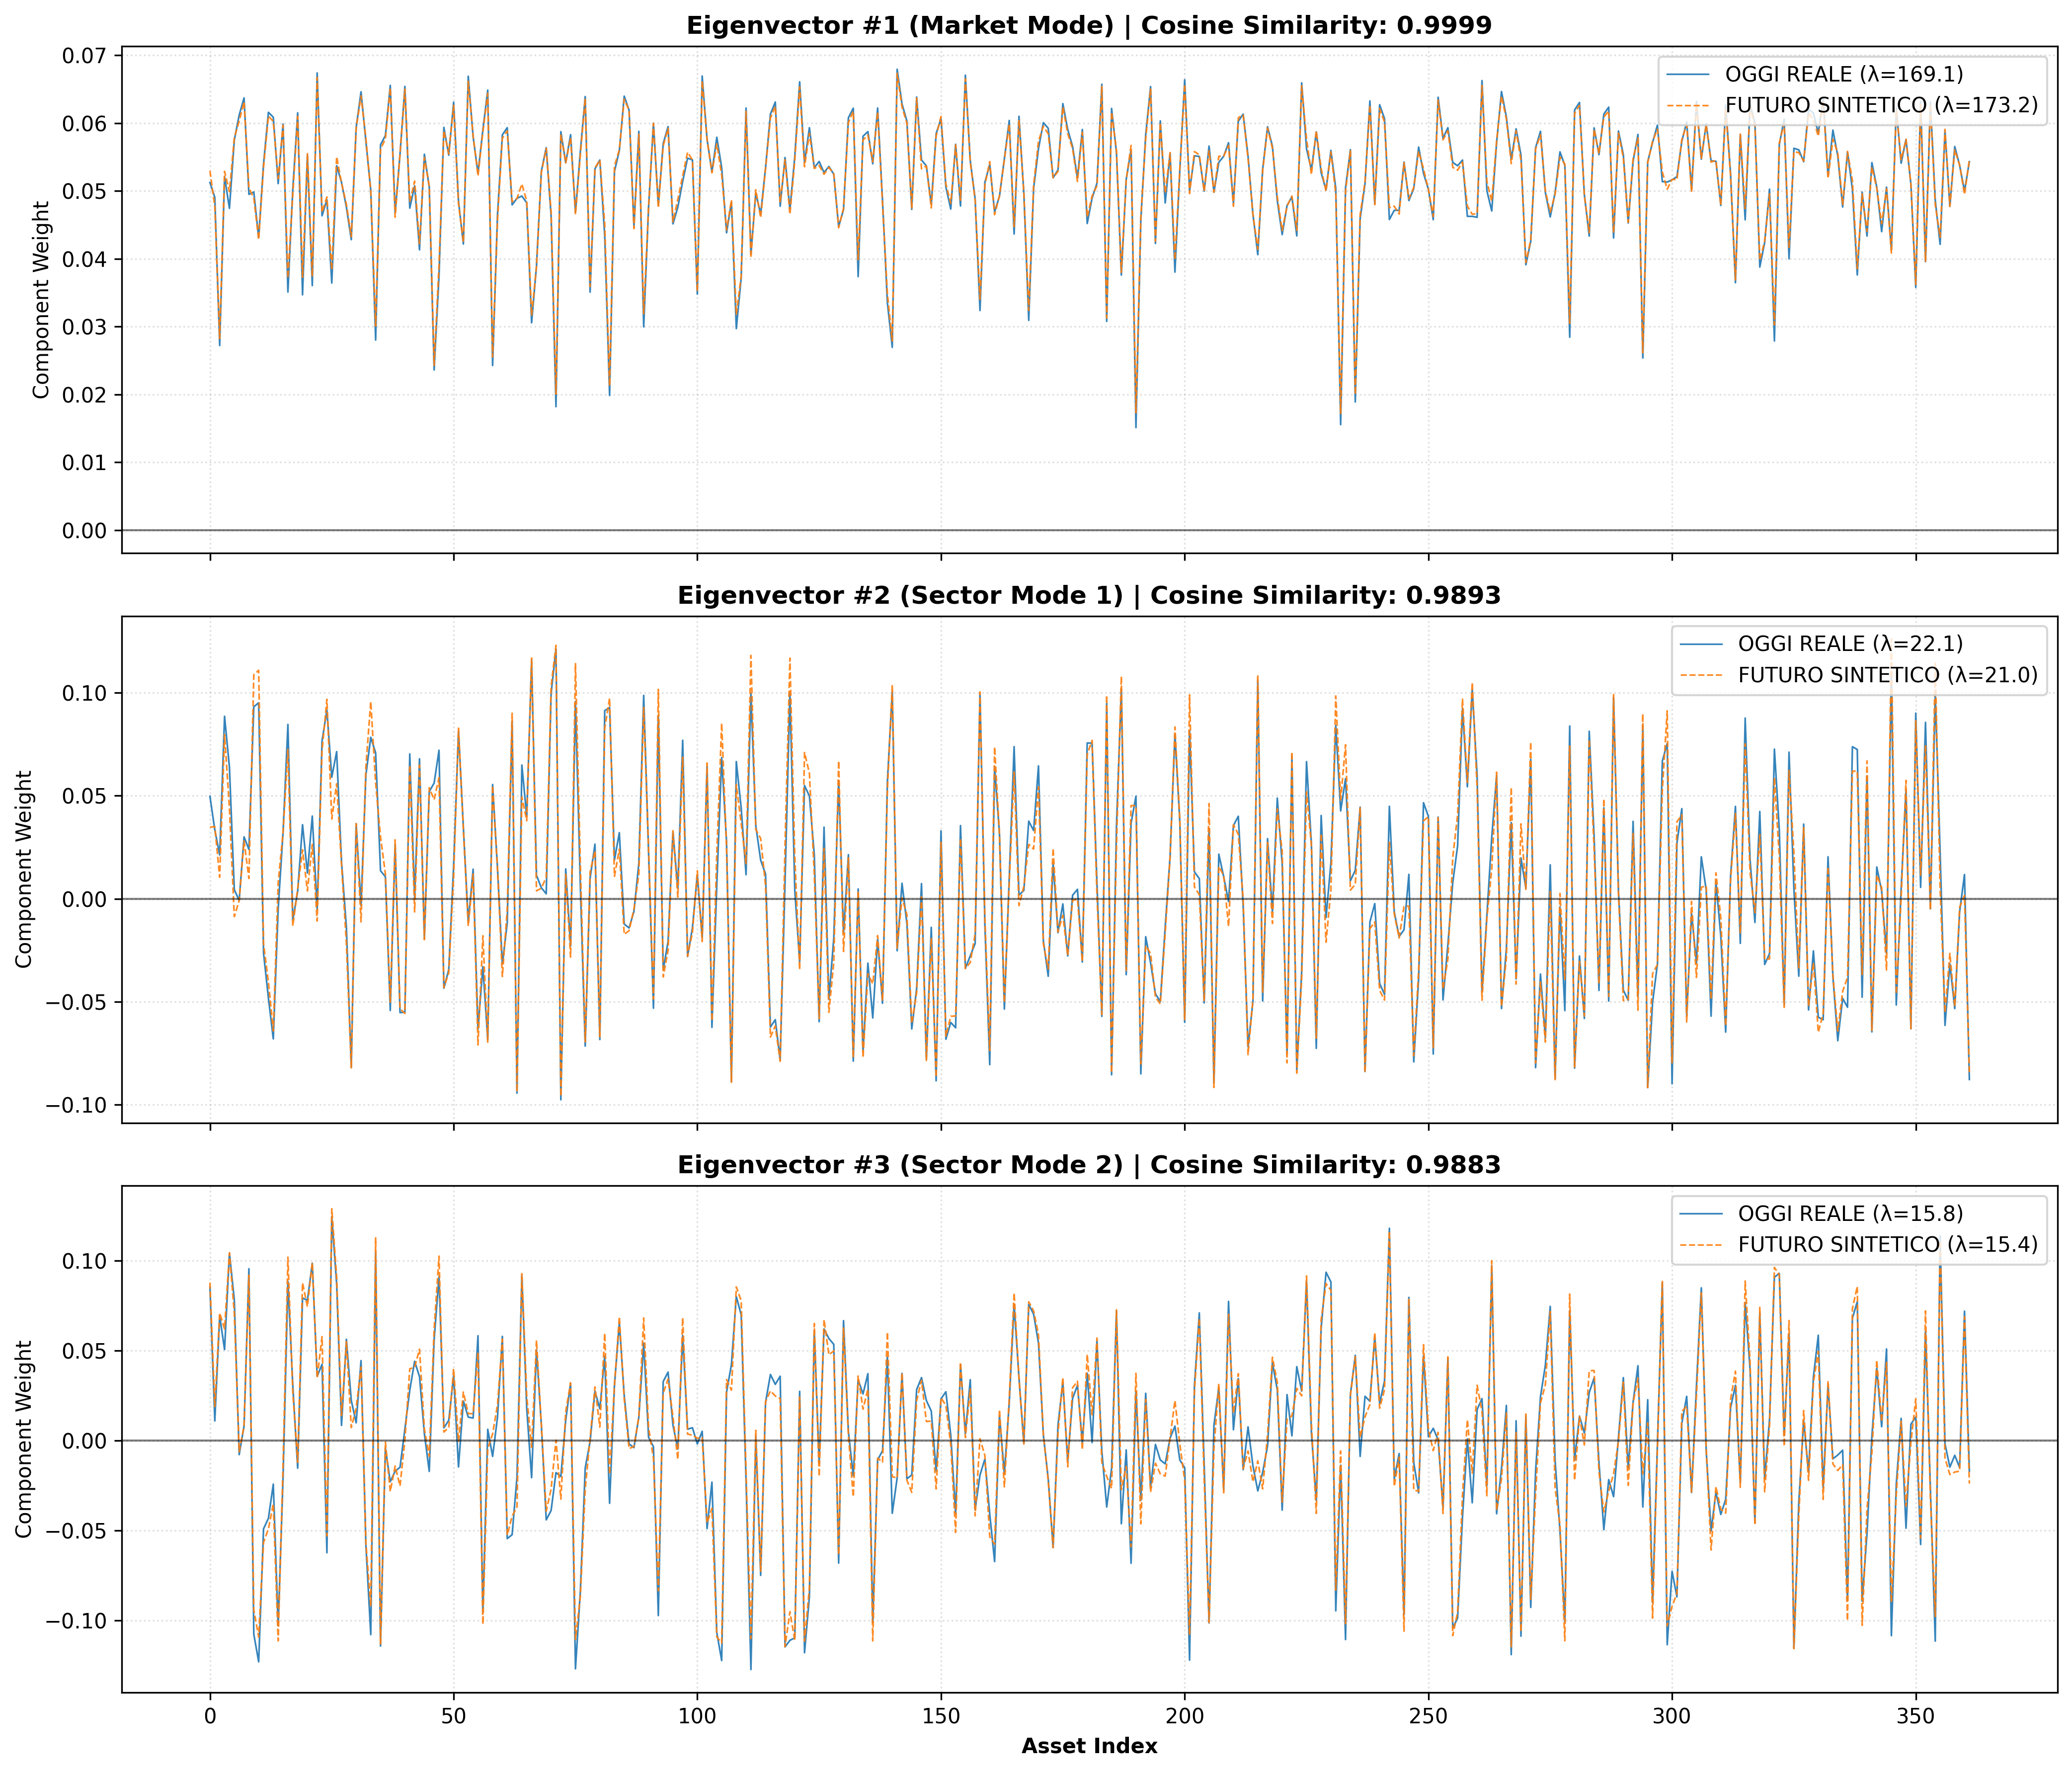
\includegraphics[width=0.85\textwidth]{./Pictures/capitolo8/fig_perron_frobenius_generato.png}
\caption{Confronto dei primi tre autovettori tra matrice odierna e matrice sintetica: le componenti del \emph{market mode} (in alto) sono tutte dello stesso segno in entrambe le matrici.}
\label{fig:pf_generato}
\end{figure}

\paragraph{Struttura gerarchica.} Il dendrogramma ottenuto per clustering gerarchico sulla matrice sintetica (Figura~\ref{fig:dendrogram_generato}) riproduce visivamente un'organizzazione a blocchi molto simile a quella della matrice odierna, con gli stessi principali raggruppamenti settoriali riconoscibili nella struttura ad albero.

\begin{figure}[h!]
\centering
\includegraphics[width=0.95\textwidth]{./Pictures/capitolo8/fig_dendrogram_generato.png}
\caption{Dendrogrammi comparativi per la matrice odierna (in alto) e la matrice sintetica a un mese (in basso).}
\label{fig:dendrogram_generato}
\end{figure}

\paragraph{Topologia scale-free del MST.} L'esponente della legge di potenza stimato sulla distribuzione di grado del Minimum Spanning Tree (Figura~\ref{fig:mst_generato}) risulta $\gamma_{\text{oggi}} = -2.119$ per la matrice odierna e $\gamma_{\text{futuro}} = -2.227$ per lo scenario sintetico: entrambi i valori confermano la natura \emph{scale-free} della topologia di rete, con un grado massimo di 15 e 14 connessioni rispettivamente.

\begin{figure}[h!]
\centering
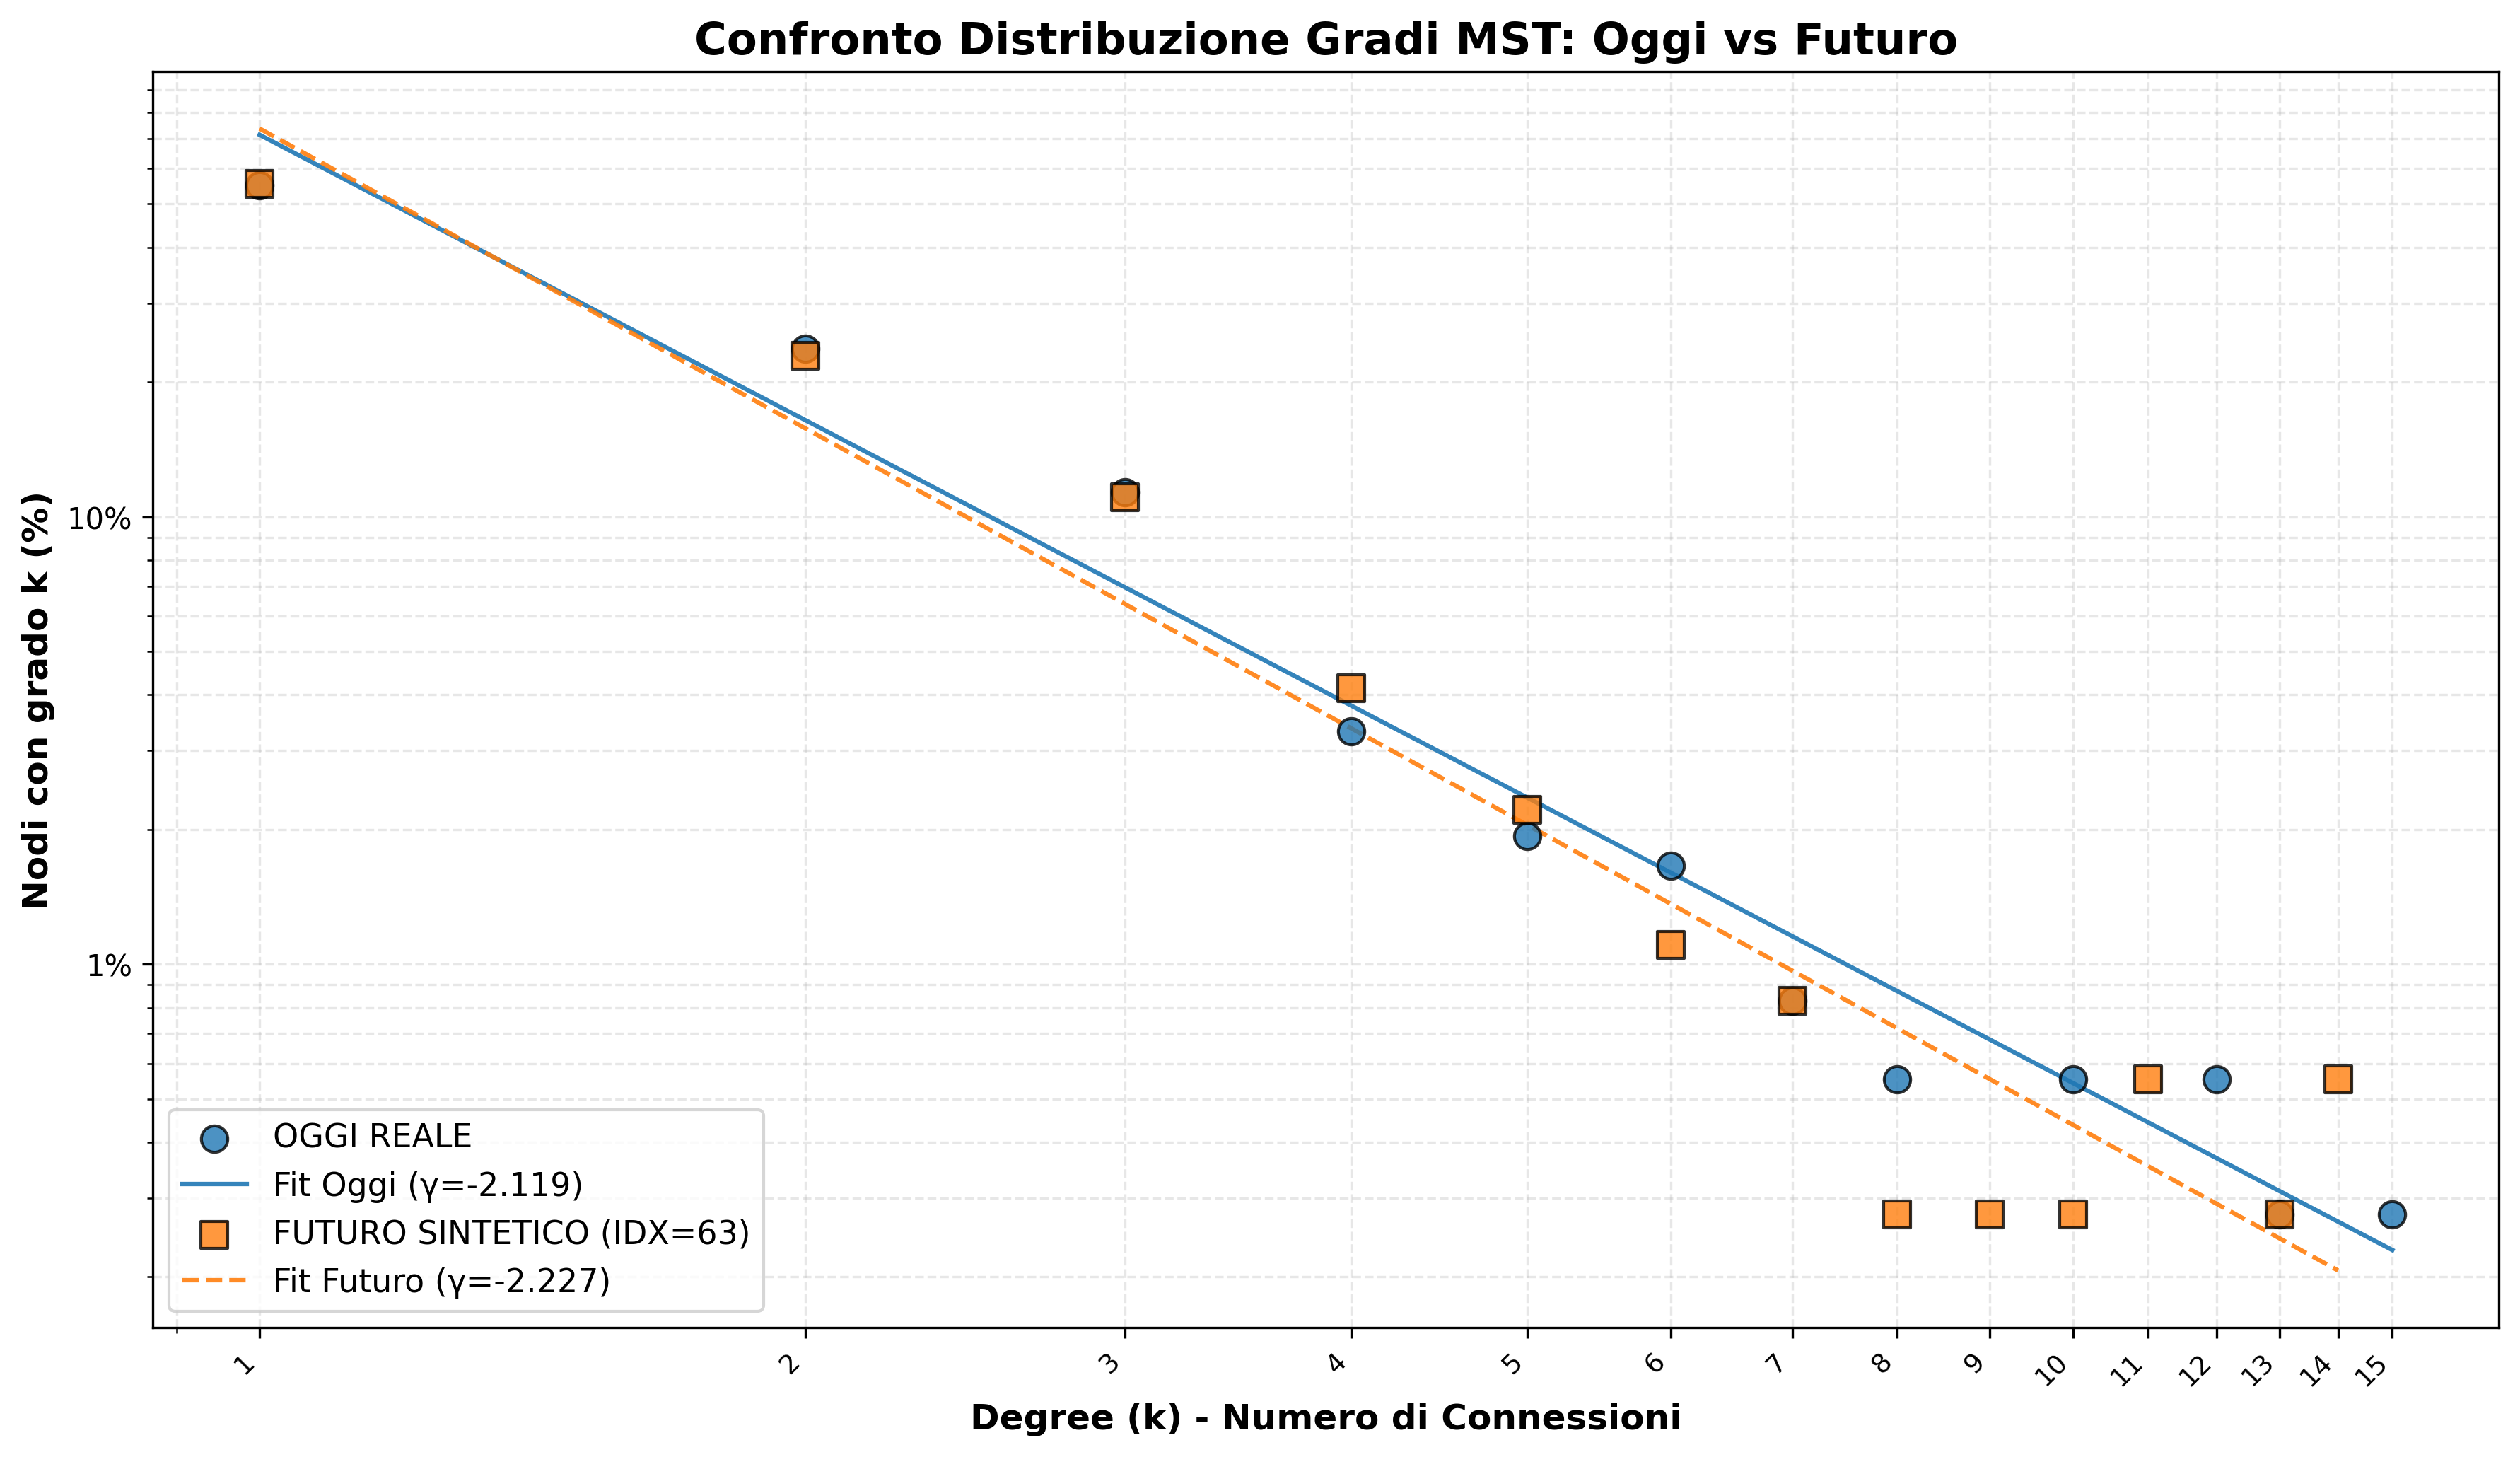
\includegraphics[width=0.75\textwidth]{./Pictures/capitolo8/fig_mst_degree_generato.png}
\caption{Distribuzione di grado del Minimum Spanning Tree in scala log-log, matrice odierna vs matrice sintetica a un mese.}
\label{fig:mst_generato}
\end{figure}

\section{Limiti della validazione e sviluppi futuri}
\label{sec:limiti_validazione}

\begin{osservazione}
La verifica presentata in questa sezione, pur non avendo evidenziato alcuna violazione dei cinque fatti stilizzati, è condotta \textbf{su un singolo scenario per volta} scelto tra i 1000 generati, e non in forma aggregata sull'intero insieme. Una validazione statisticamente più esaustiva richiederebbe di ripetere l'analisi (o quantomeno le metriche riassuntive: percentuale di scenari con proprietà di Perron-Frobenius soddisfatta, distribuzione dell'esponente $\gamma$, istogramma \emph{pooled} delle correlazioni \emph{pairwise}) sull'intero insieme di scenari generati, anziché su un singolo campione rappresentativo. Questo approfondimento è lasciato come sviluppo naturale del presente lavoro.
\end{osservazione}

Le matrici sintetiche generate in questo capitolo, avendo superato la verifica qualitativa sui cinque fatti stilizzati, costituiscono un insieme di scenari plausibili pronti per essere utilizzati come input di un motore di simulazione Monte Carlo per l'\emph{asset allocation} e la gestione del rischio di portafoglio (ad esempio per la stima del Value at Risk o dell'Expected Shortfall, sul modello di \citet{caprioli2024ptfvae}) --- applicazione che, per scelta di perimetro, non è stata affrontata in questo lavoro e viene proposta tra gli sviluppi futuri nelle Conclusioni.
